\chapter{Methodology}\label{Methodology}
In this chapter the data mining methods used to retrieve movement patterns from the TU Delft eduroam Wi-Fi log data will be described in detail. \autoref{figure:workflow} gives an overview of the main workflow to derive movement patterns from the Wi-Fi log. First the raw Wi-Fi log is preprocessed to get states at two different spatial levels (building- and building-part level). A state is defined as a time interval during which a particular device is located in a certain area. An example of a state on building level is: device A is located at Library from 11:00 to 12:00. An example on building-part level is: device A is located at canteen from 11:00 to 12:00. In the preprocessing phase the data is enriched with 'world' states, reduced by grouping states and cleaned by filtering out 5 minute states representing people that only pass by a building without actually entering it. The insertion of world states enables the detection of movement from and to the campus in the case of building level, and movement from and to the building in the case of building-part level. The assumption made here is that the device is not switched off. Especially in the case of laptops it is likely that the device is switch of for some hours during a lecture for example, this could be interpreted as a movement off campus. Therefore a mobility analysis is conducted attempting to distinguish between mobile phones and laptops, which are the two main device categories present in the dataset. The states resulting from the preprocessing are used to retrieve movements at both spatial levels. A movement is defined by the change from one state to the next subsequent state, where the different states must be at a different locations. Furthermore, the building level states are used to retrieve trajectories for each device. A trajectory is defined as an ordered list of states. The trajectory thus stores the entire route or trajectory the particular person travelled. For the building-part level no trajectories are retrieved. For building-part level a graph is made for BK-city. In this graph the nodes represent the different building-parts and the edges follow movement space, such as corridors and stairs. Using the shortest path in the graph, the route of the movements within BK-city can be visualized in more detail. For building level no graph is created, therefore the trajectories and movements are visualized simply as a straight line. In addition to the maps at both the building and building-part spatial level, movement time series are created for both spatial levels. Together these maps and time series are used to identify different types of movement patterns.

\begin{figure}[H]
\centering
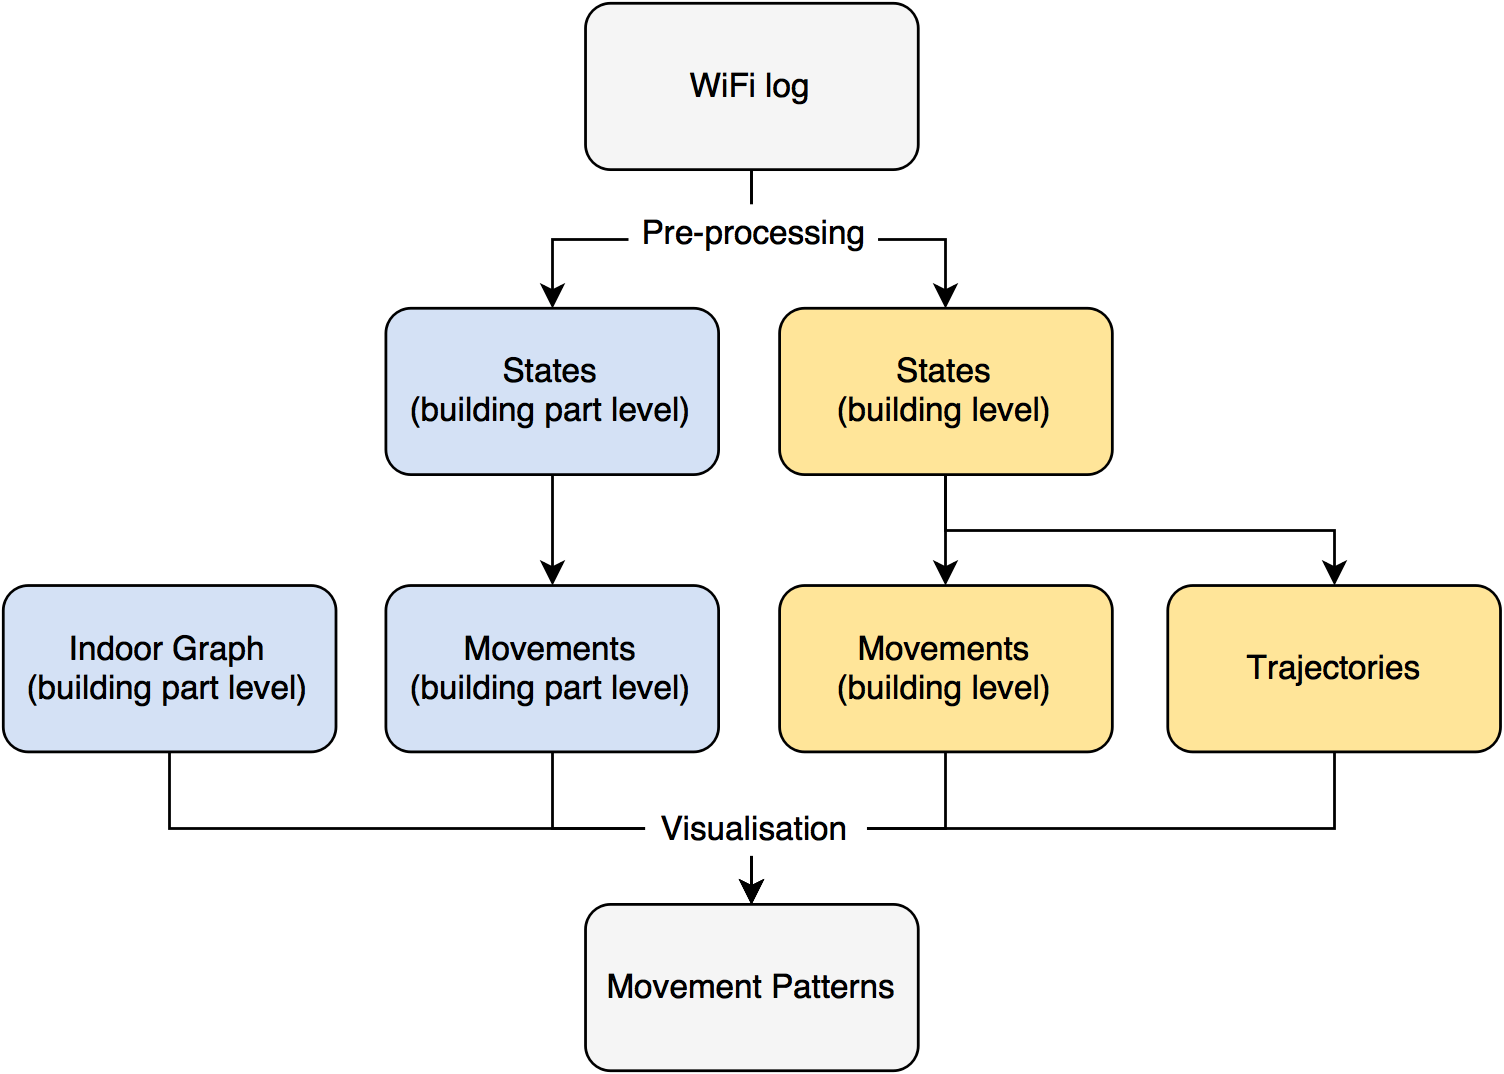
\includegraphics[scale=0.25]{methodology_workflow}
\captionsetup{justification=centering}
\caption{Grouping}
\label{figure:workflow}
\end{figure}
In the following sections all steps to derive movements and trajectories from the Wi-Fi log will be described in more detail. First \autoref{preprocessing} describes the various pre-processing steps to clean, reduce and enrich the raw data. \Cref{mobility} will describe the mobility analyses which aims to distinguish between laptops and mobile phones. Subsequently \autoref{statesToMovements} addresses how the movements are retrieved from the states for both spatial levels. Finally \autoref{statesToTrajectories} describes how the trajectories are created from the building level states. In \autoref{movements} to \autoref{indoormovement} the visualisation and results of the movements and trajectories are addressed, for building-part level this also includes creation of the graph. 

\section{Preprocessing}\label{preprocessing}
Before movement patterns between buildings and building-parts can be retrieved, pre-processing of the raw data is required. In this chapter the different pre-processing steps will be described in detail. First \autoref{initialfiltering} addresses the initial data filtering. \autoref{grouping} concerns the grouping of records with the same mac address and location that are subsequent in time. \Cref{addingWorld} describes the filling of the dataset with a ‘world’ location. This enables detection of movement from and to the campus on the building level, and movement from and to the building on building-part level. Finally \autoref{passingBy} is about the filtering of records of people only passing by a building or building-part.

\subsection{Initial filtering}\label{initialfiltering}
Each record in the wifilog represents the scanning of a certain device at a certain time by a certain access point. In order to detect the movement patterns of these devices between buildings it should be known for each access point in which building it is located. The data in the table 'wifilog' contains information about the location of the Access Point (AP) in two columns. The first column which contains information about location, is the column 'maploc'. This column contains strings, which look as follows: 
\\
'System Campus \textgreater [buildingid] \textgreater [specific location]'. An example of such a string is 'System Campus \textgreater 21-BTUD \textgreater 1e verdieping'. In such a string, the middle part can be linked to a building, so to a real-world location. But there are some other values for maploc, which can less clearly be linked to a real-world location. Such a value is 'Root Area', it is unclear what this value means and it contains no information about a building or area it might be in. This makes it impossible to link it to a location in the world. Then there is the value 'Unknown', a value that indicates that there was no name attached to the Access Point that user was connected to. Again in this case, it is impossible to link this value to a real-world location. As both 'Root Area' and 'Unknown' are in the minority of records, they could be left out of the queries, but this would mean removing many records from the dataset, which is not desired.
\\\\
The second one is the column 'apname', which is a string with the symbolic name of the AP, for example 'A-08-G-010'. The two numbers in the second part of the string, in this case '08', represent the building number. This building number can be linked to a location in the world. In some cases, the column 'apname' did provide information about the location, while the 'maploc' column value was unclear. In most of these cases however, the building number, the second part of the string, was a three digit number. But there are no buildings on the TU Delft campus with a building number that high. When consulting Wilko Quack about this, he explained that these building numbers had an arbitrary 1 in front of the building number. So 'A-134-A-001' was not building 134, but building 34, which was an actual building number on the campus. This would mean that using the column 'apname' for getting the building number would mean a higher number of results and therefore a more realistic visualization of the movements. Two other special cases are present in which the building id in the apname is 102 or 104. These ids corresponds to the legermuseum and the VLL-LAB respectively. As the legermuseum in not located on the campus it was decided to omit this building. The VLL-LAB did have no building number according to the TU Delft Campus maps, which was why the building was not identified before. After finding this, the building was manually added to the buildings table.
\\\\
The information about the location is linked to the actual locations of the buildings using the buildings table. Each building has an id, name and geometry. The id is taken from each record using a Python function and linked to the id in the building table. The building-part tables works in the same way, but then every full apname from a record is linked to the corresponding building-part.

\subsection{Grouping of states}\label{grouping}
In order to reduce the data and to be able to filter out records of people only passing by a building, the data needs to be grouped. The overall goal is to identify movement patterns between different buildings or building-parts. As a result records of subsequent states of the same device in the same building or building-part can be grouped together into one single record. Namely, if two subsequent states are at the same location they do not represent a movement and can thus be grouped. When looking at building level, the mobile of someone who studies the whole day at architecture might have 20 records (states) in the database for that day. This can be reduced to one record (state) that contains the time the device arrived at Architecture and left again. For building-part level the same applies for someone that has multiple subsequent states in the same building-part. To determine whether two records are subsequent in time, and therefore should be grouped together, a threshold for the time gap between two records needs to be defined. It was decided to set the gap threshold for grouping states to 1 hour. The reasoning behind this is that someone who is not scanned for a period of more than 1 hour has likely left the building. However, if someone is away for less than an hour it more likely that that person was just smoking or lunching outside or just disconnected for from the system for a while. \autoref{figure:grouping} gives an example of how the records are grouped on building level for one device for one single day. It should be noted that two states remain at faculty A as the gap between 12:30 and 13:45 is bigger than an hour. In the other other cases the gap is smaller than an hour and the records are grouped together. Only one records is present at faculty B so this record can not be grouped. The grouped records still contain all the information that is required to know that the person moved from faculty A to B to C during the day. 

\begin{figure}[H]
\centering
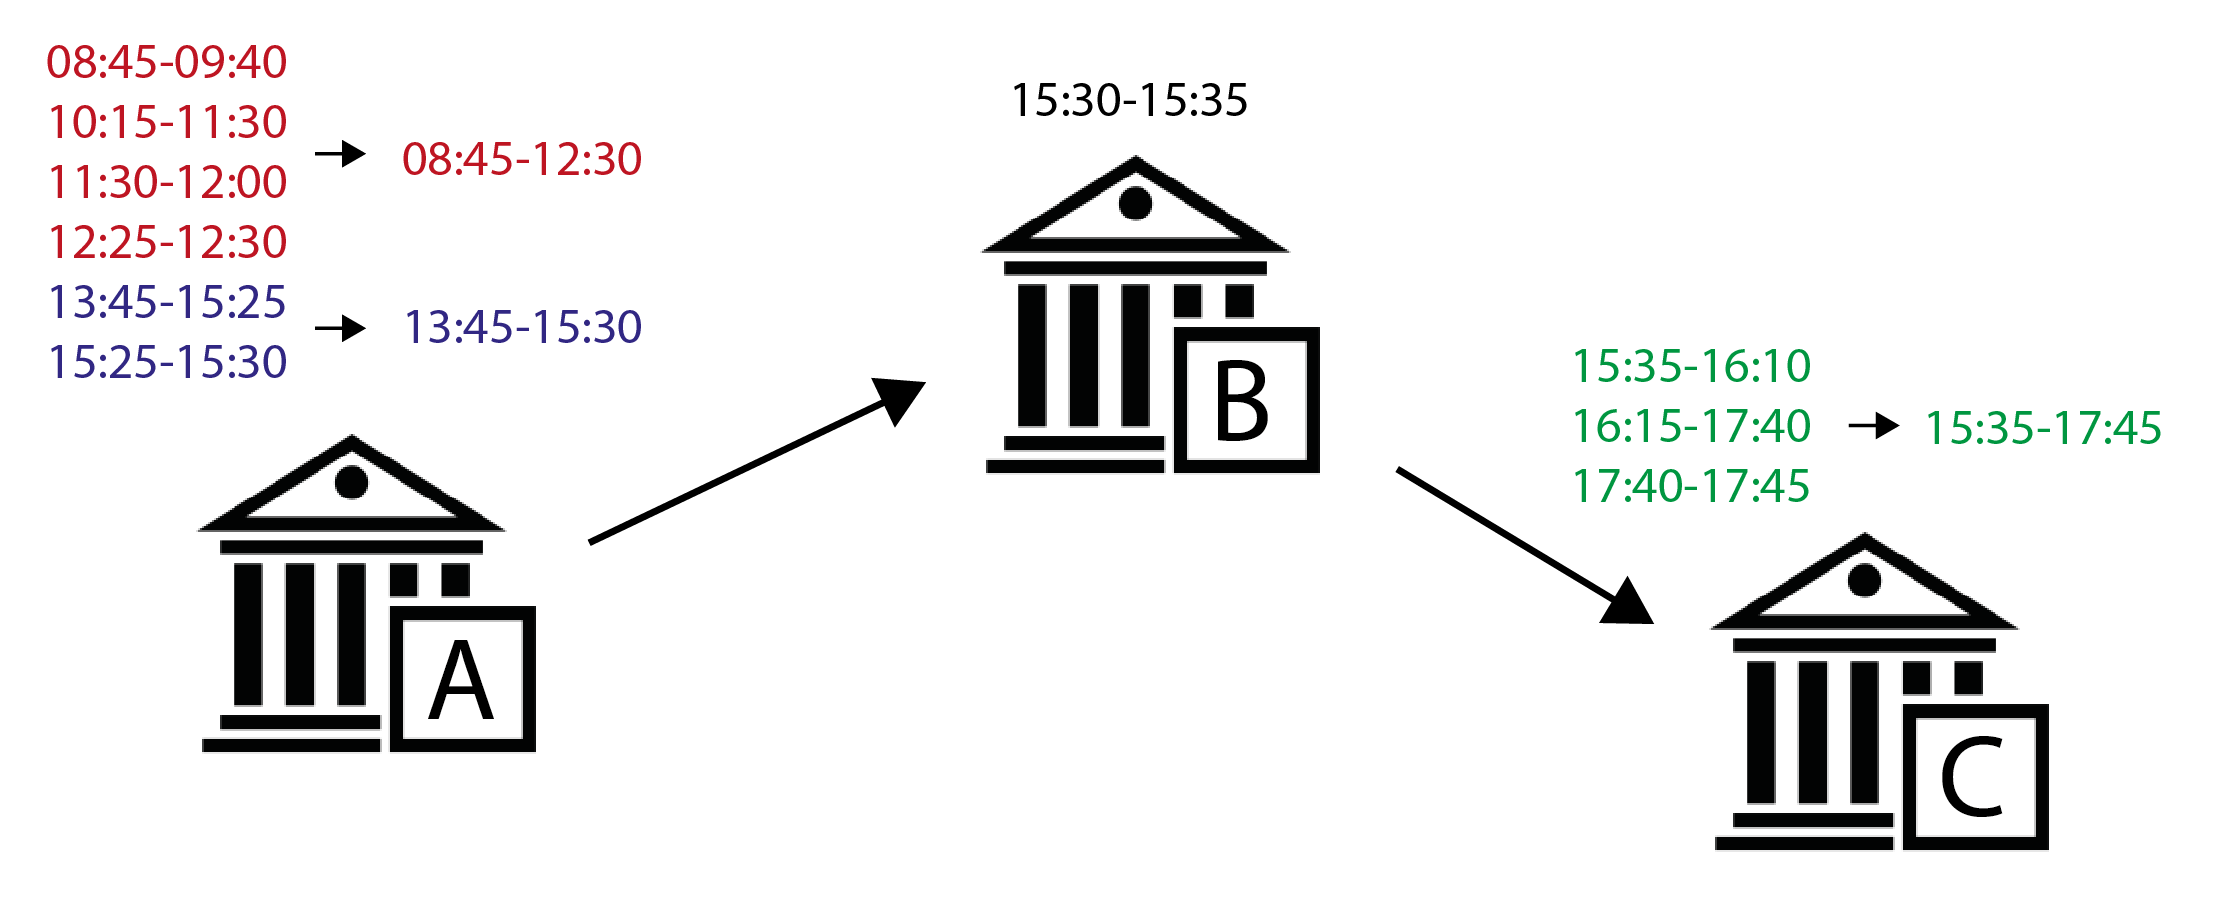
\includegraphics[scale=0.7]{Preprocessing_Grouping}
\captionsetup{justification=centering}
\caption{Grouping}
\label{figure:grouping}
\end{figure}

\subsection{Adding world state}\label{addingWorld}
Because the dataset contains all records of when certain devices are scanned, it also Implicitly stores information on when the device is not located at the campus. These time gaps in which a particular device is not scanned at the campus give information on when the corresponding person is not at the campus. This information is valuable for detecting movement patterns from and to the campus in addition to the movement between buildings at the campus. Considering the fact that many student only visit one faculty each day. It becomes especially clear, that the movement from and to the campus plays an important role in the overall movement pattern of a person. In order to be able to directly derive movement from and to the campus from the dataset, the time gaps present in the data should be stored explicitly. Therefore each time gap larger than an hour is filled with a outside campus or 'world' record. The word 'world' is used to indicate that the device could be located at any place in the world outside the campus during the time spans that it is not scanned at the campus. It should be noted the reason that a device is not connected to one of the access points could also be that the device is simply switched of, in this case however the assumption is made that the device moves off campus. The begin and end time of a world record is defined by the end of the previous record and the start of the next record in time. In case there is no previous or next record the boundaries are defined by the starting time of the whole dataset and the current time. \autoref{figure:world} visualizes the explicit storing of world states that fill time gaps during which a device is not recorded on campus. In can be seen that three 'world' states are added in the example. First during the start of the day before the person goes to faculty A, second during the lunch break, and finally in the end of the day starting from the moment when the person leaves faculty C. Storing these world states explicitly enriches the data as much more movement can be defined. The grouping of records described in \autoref{grouping} and adding of a world state are complementary. If the gap between two states is smaller than an hour they are grouped if the gap is bigger than an hour a world state is inserted. For the building-part level the insertion of world states works exactly the same. In this case however the world represent the outside building area instead of outside campus area.

\begin{figure}[H]
\centering
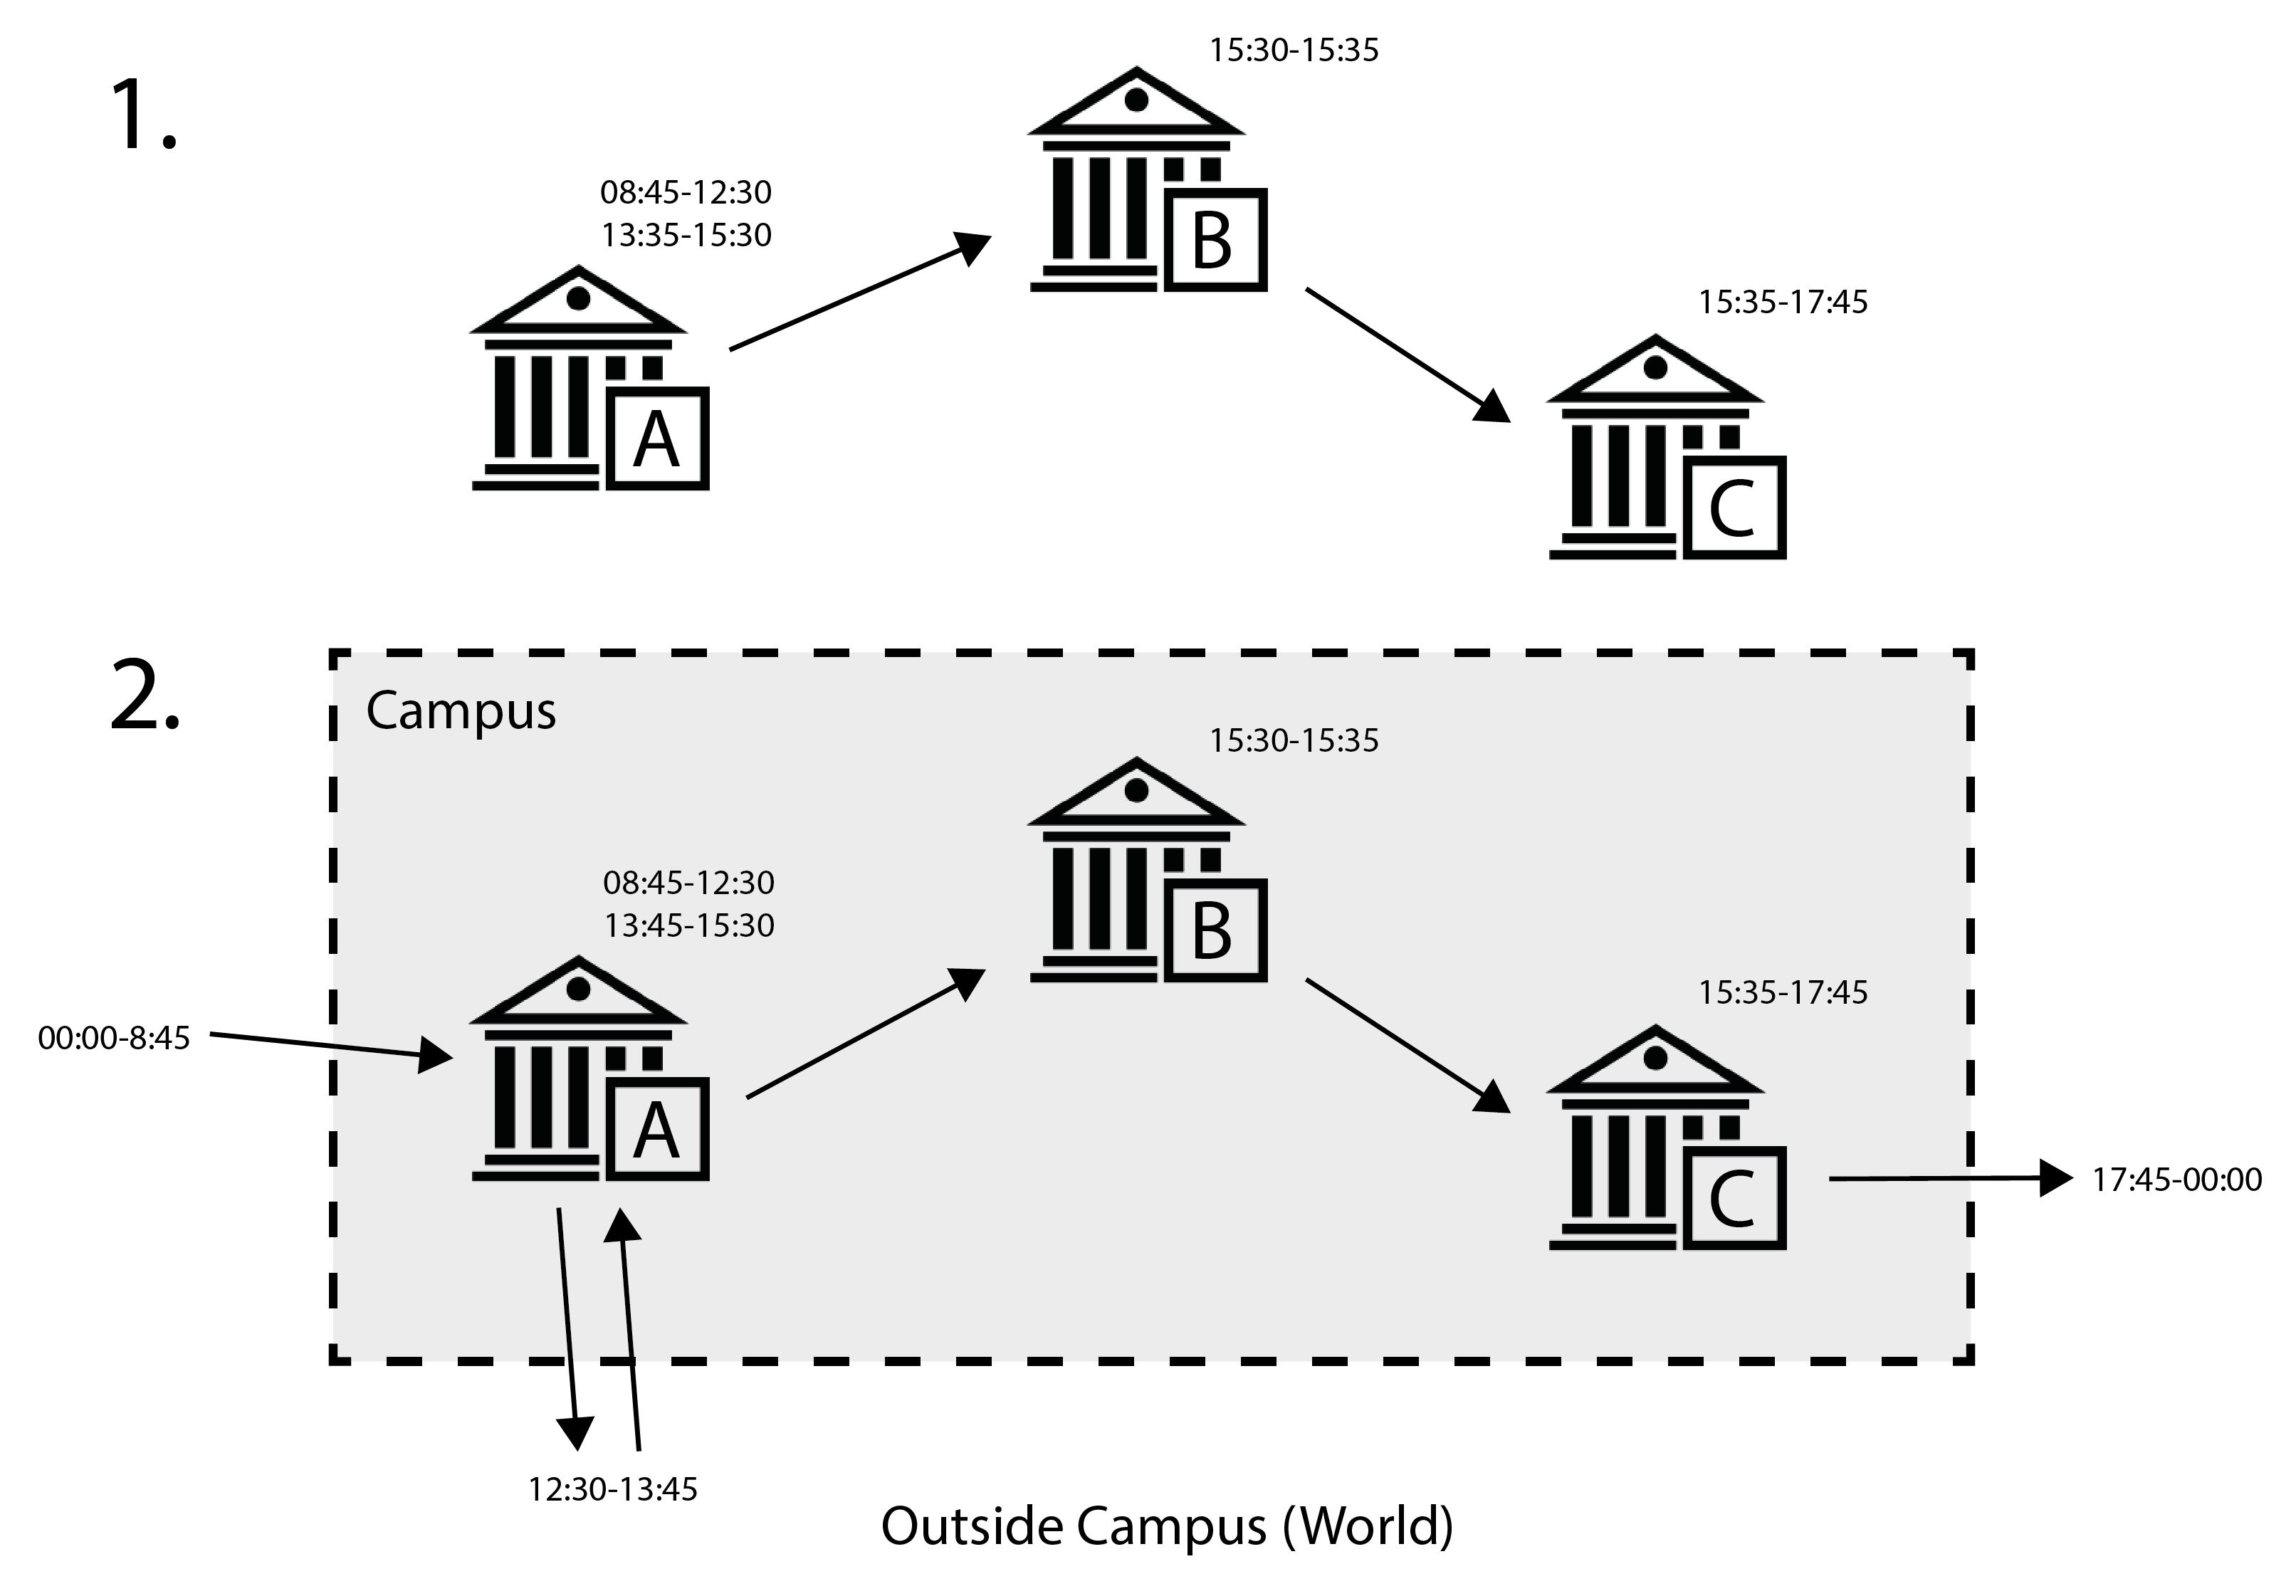
\includegraphics[scale=0.57]{Preprocessing_World}
\captionsetup{justification=centering}
\caption{Adding World}
\label{figure:world}
\end{figure}

\subsection{Passing by}\label{passingBy}
For the detection of movement patterns between buildings, records of people that only pass by a building without actually visiting it should be excluded. The reason for this is that records of people only passing by a building could result in misinterpretation of the movement patterns. This is illustrated by the example in \autoref{figure:passing by}. In this case faculty B is located on the route from faculty A to faculty C. Therefore it is likely that people moving from faculty A to faculty C are picked up by a scanner located at faculty B. The eduroam system records all devices at intervals of approximately 5 minutes as explained in \autoref{datadescription}. Such a recording by the eduroam system can happen during the short time period that the device, which is on its way from faculty A to C, is connected at faculty B. This will result in records of approximately 5 minutes at faculty B, whilst the person has not been inside faculty B. As the movement is the change between two states, the movement to faculty C will origin from faculty B. Someone that is not aware of the 'passing by' problem might conclude that people from faculty B often go to faculty C. In reality however, people from faculty A go often to faculty C. By filtering out the records of people only passing by buildings the correct movement can be visualized (see \autoref{figure:passing by} bottom). It should be noted that filtering out 'passing by' records can only be done after the grouping process. The reason for this is that 5-minute records that would individually be classified as someone passing by might be grouped together into one record with a longer duration. After grouping the combined record is not classified as someone who passes by anymore. Furthermore it should be noted that the filtering of 'passing by' records occurs after filling the data with 'world' states. The reason for this is that a passing by event does mean that the device was located on the campus. The world records are meant to represent the time the device is not on the campus. Filtering passing by events works exactly the same for the building-part level. If a person only passes by a particular building-part without staying in it, it is filtered out. For building-parts this filtering is especially important as the route from one building-part to another often leads through several other building-parts. 

\begin{figure}[H]
\centering
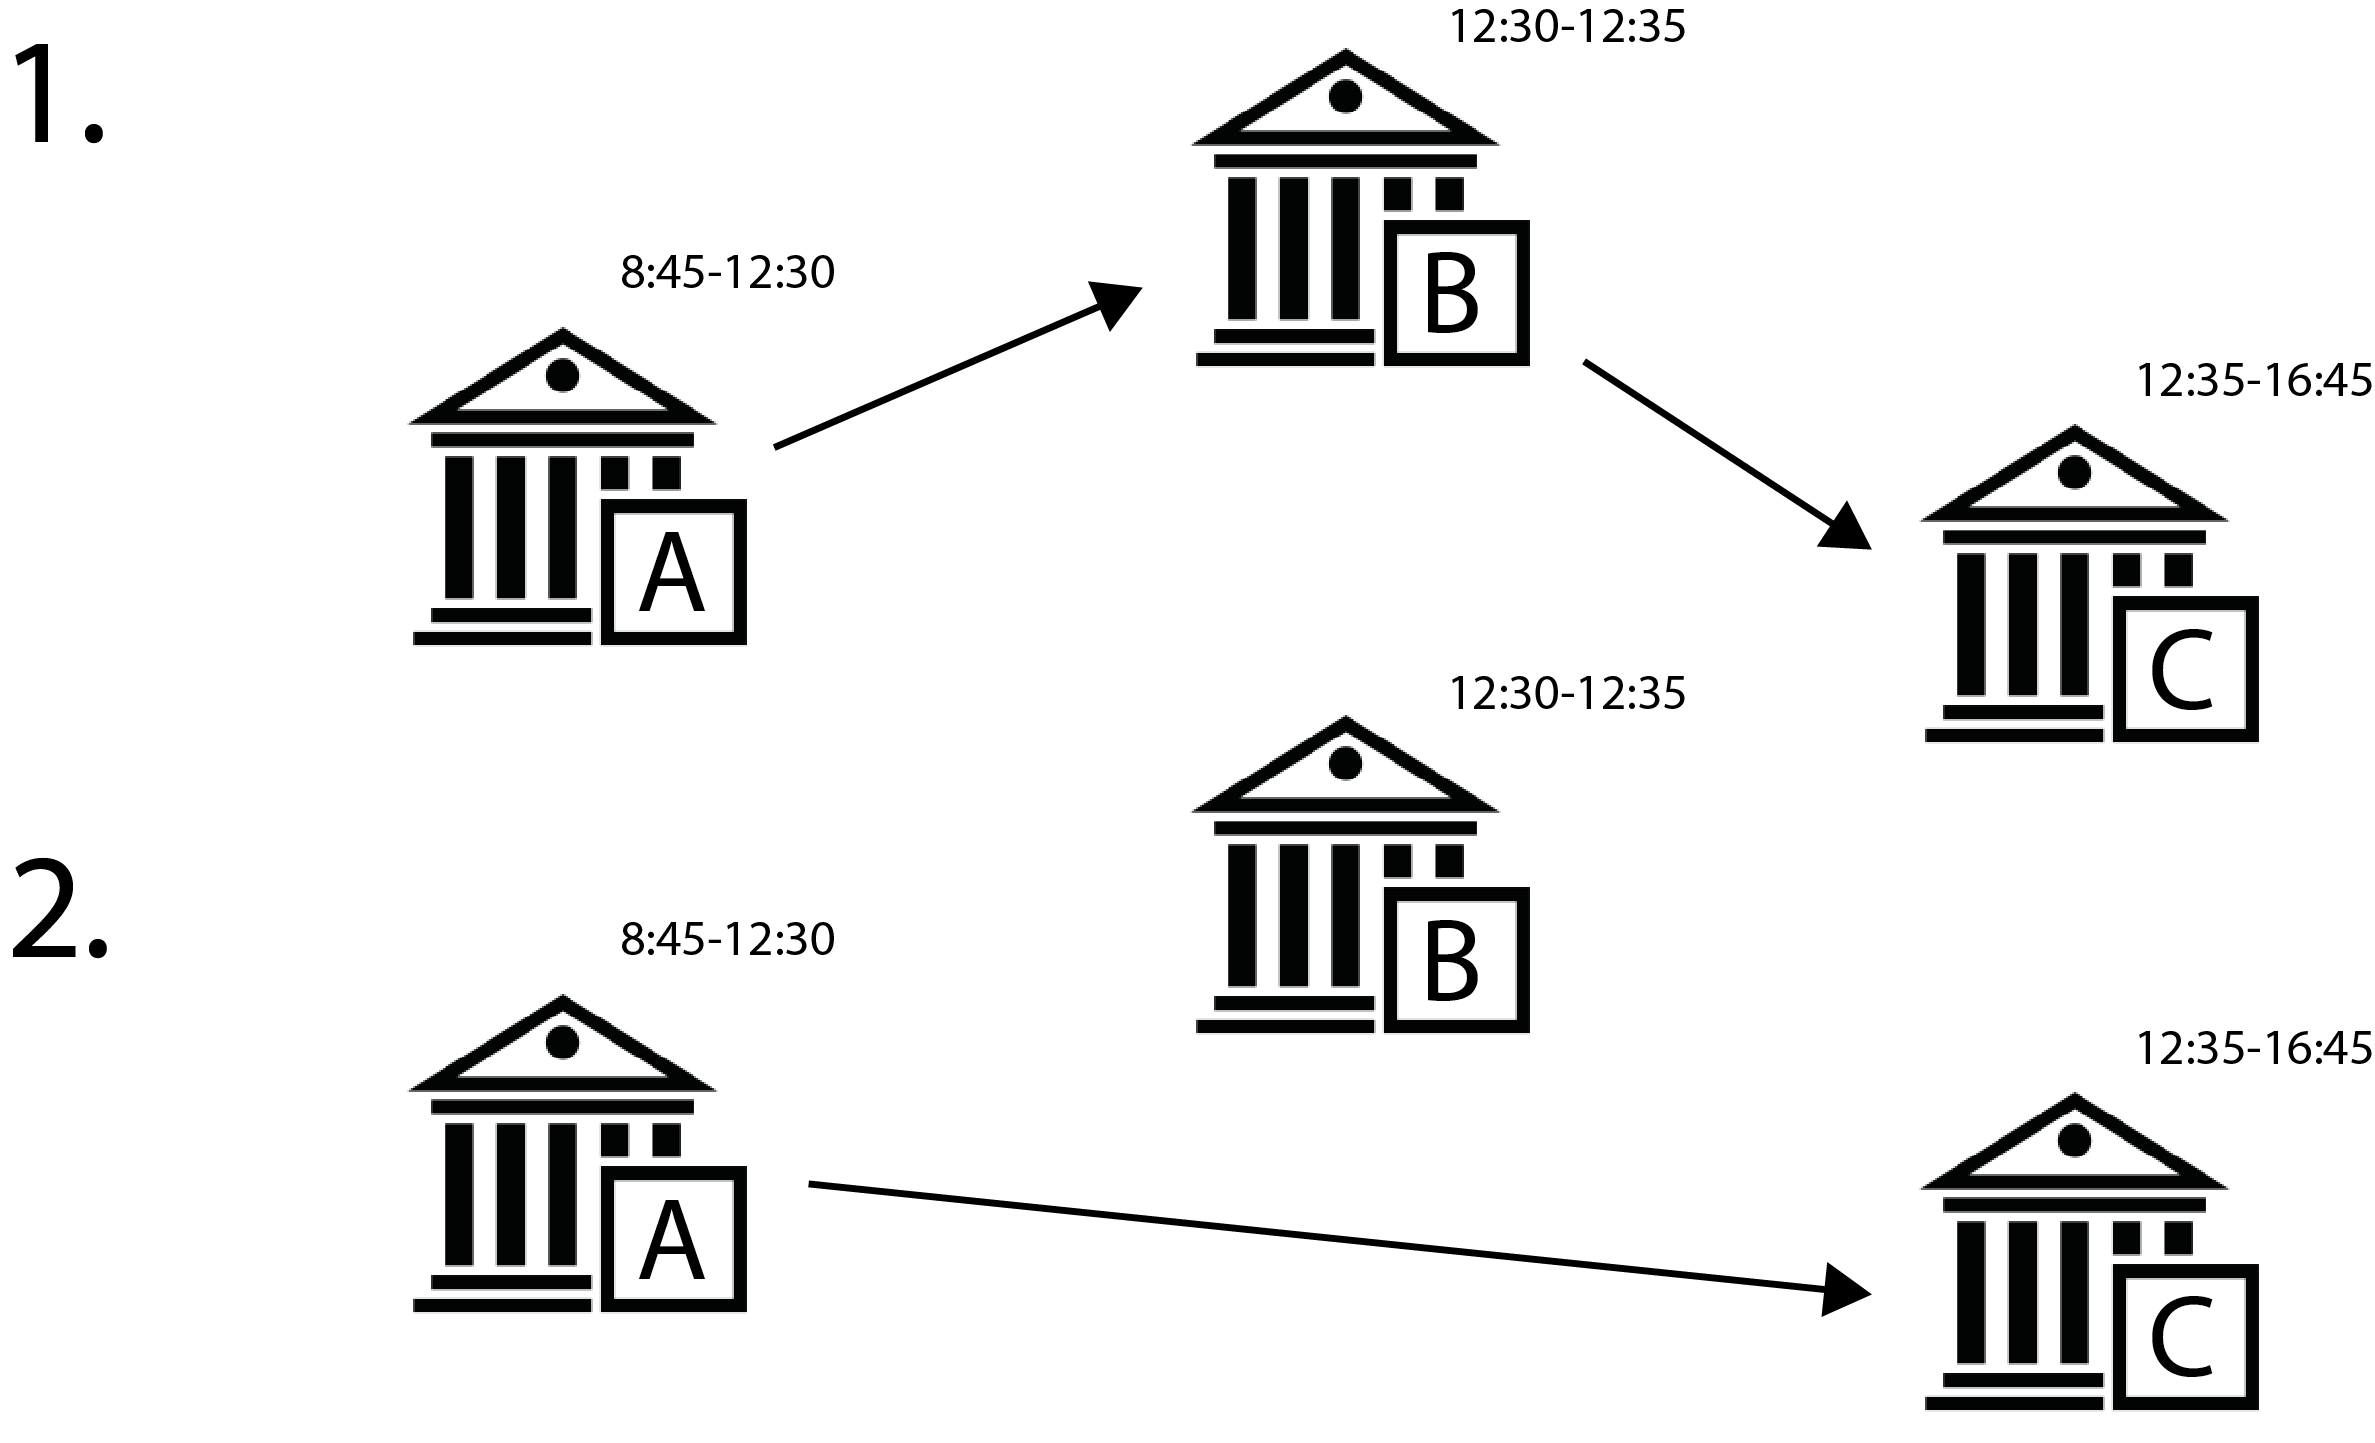
\includegraphics[scale=0.7]{Preprocessing_PassingBy}
\captionsetup{justification=centering}
\caption{Passing by}
\label{figure:passing by}
\end{figure}

\subsection{Implementation}
The filling (world), grouping and filtering (passing by) steps described above are implemented in an integrated way. The pseudo code for the implementation for building level is shown in \autoref{figure:pseudocode}, for building-part level the implementation is exactly the same only grouping is done for building-parts instead of buildings. As can be seen in the code there is communication with the database at several points. The table from which the records are retrieved for each mac address is already processed as described in the general filtering section. Furthermore the format of the table is slightly different compared to the initial wifilog. The session duration is exchanged for an end time column which is derived by adding the session duration to the asstime (start time of a record).

\begin{figure}[H]
\centering
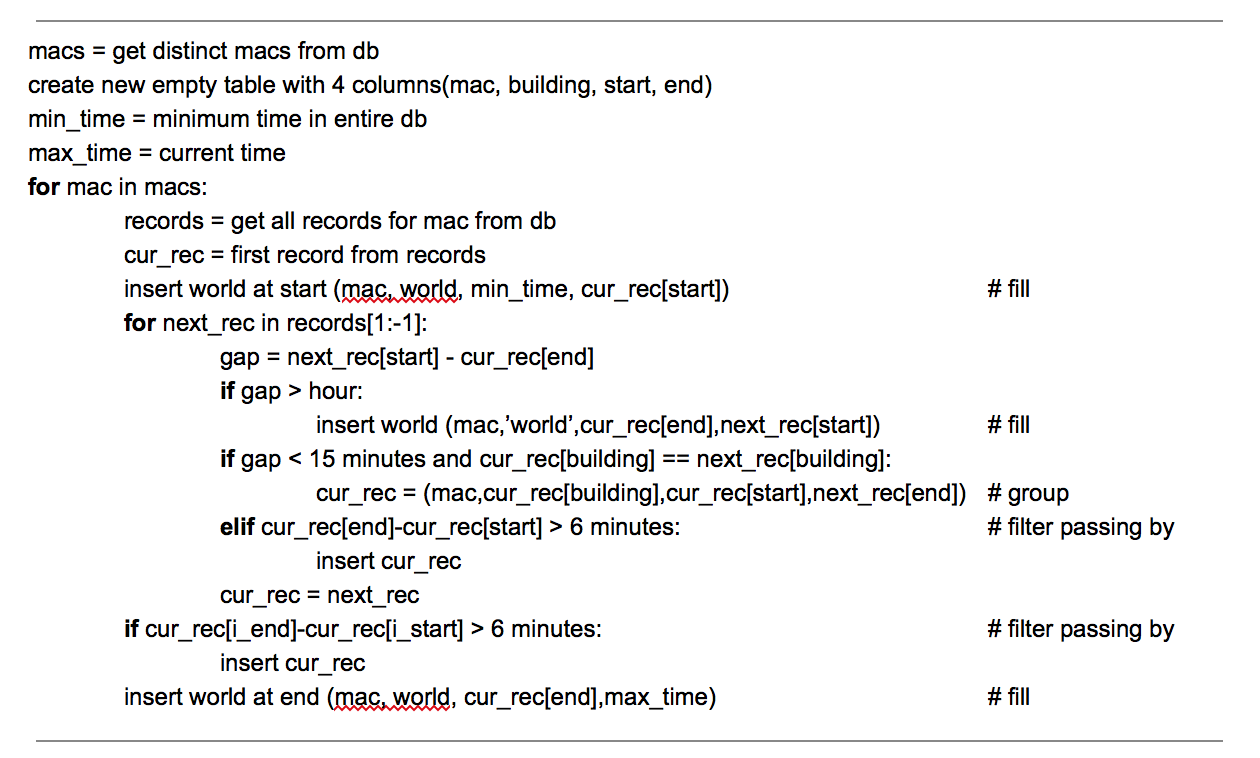
\includegraphics[scale=0.5]{pseudocode.png}
\captionsetup{justification=centering}
\caption{Pseudocode preprocessing}
\label{figure:pseudocode}
\end{figure}

\autoref{figure:Preprocessing} shows an example of the records of one device over a time span of one day during the different pre-processing steps. From the raw data it can be seen that this person spends most of the day in building B. The person is scanned once at building A before he arrives in the morning and after what is likely to be his lunch break. The last two hours the person is scanned in building C. After filling three world records are added, at the beginning of the day, during the lunch break, and at the end of the day. The grouped records show that the subsequent scans in building B and C are grouped together. Finally the scans at building A are removed from the dataset as they are likely to indicate passing by events. 

\begin{figure}[H]
\centering
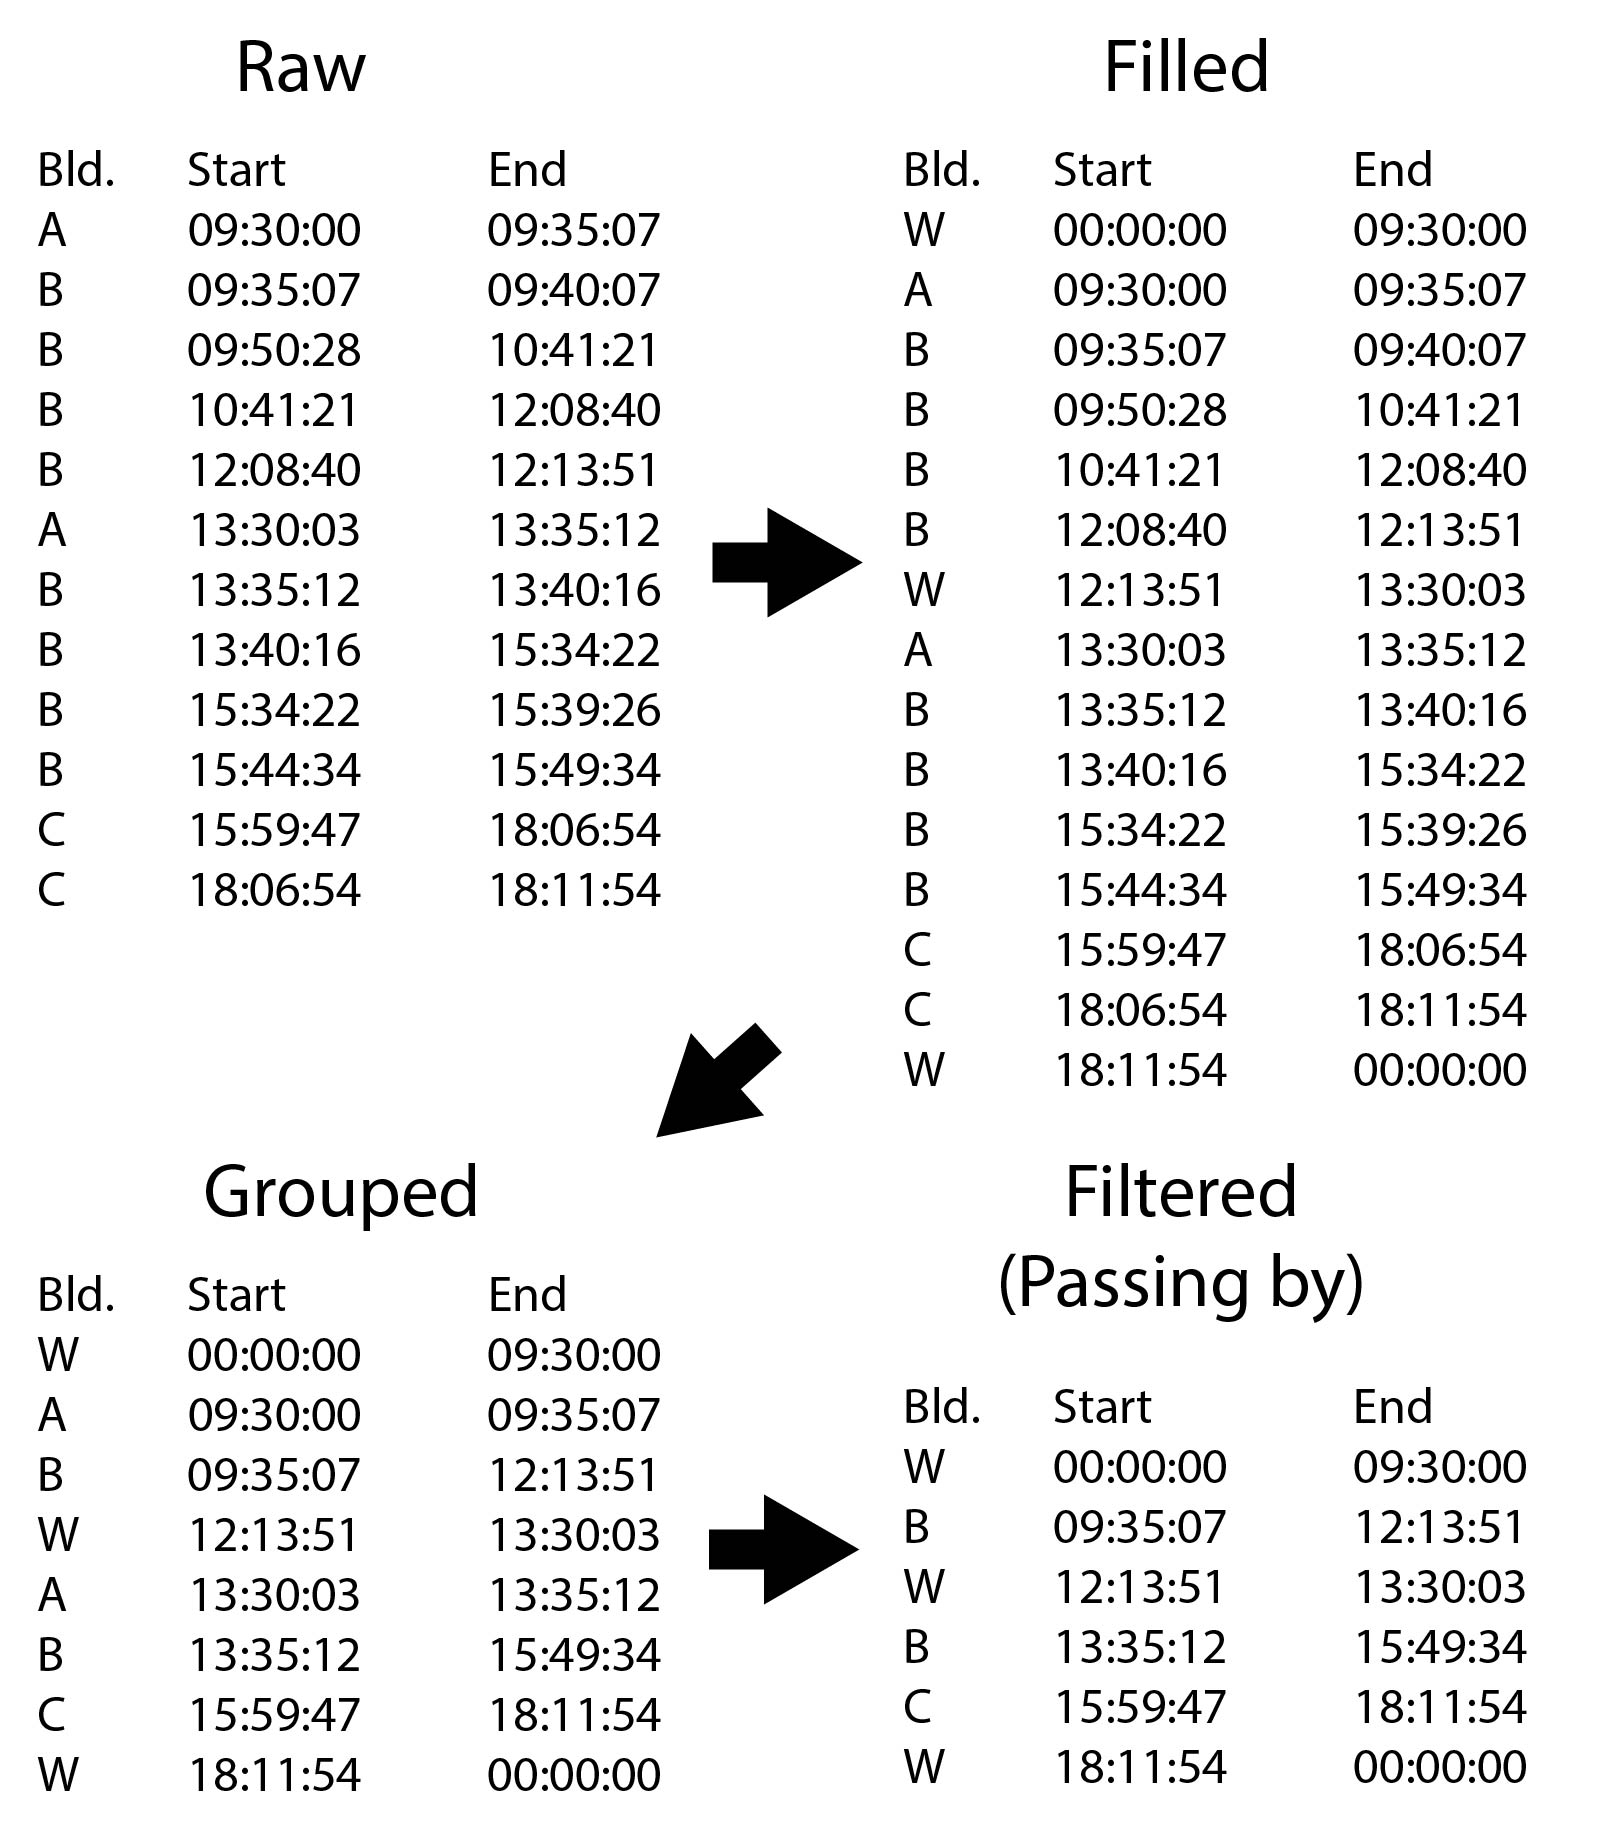
\includegraphics[scale=0.2]{PreProcessing-01.jpg}
\captionsetup{justification=centering}
\caption{Preprocessing}
\label{figure:Preprocessing}
\end{figure}

\section{mobility analysis}\label{mobility}
As described in \autoref{addingWorld} gaps in the data during which a device is not scanned are filled up with world states. It is however possible that the reason a device is not scanned at the campus is not because the device left the campus, but simply that the device is switched off or lost connection to the network. Especially in the case of laptops it is likely that several gaps in the data are present, due to the fact that the particular person closes its laptop for example to have lunch or go to a lecture. Furthermore it is likely that the laptop is only opened when the person starts studying and not when the person is actually entering the building. Mobile phones on the other hand are likely to have fewer gaps in the data as they are usually not switched of during the day. In terms of movement the results could be more accurate by filter out the laptops and only looking at mobile phones. Furthermore distinguishing between mobile phones and laptops enables comparison of the movement patterns of the different device types. 
\\
The main difference between laptops and mobile phones is that laptops are usually on switched on if a person is stationary at a certain location. Mobile phones on the other hand are usually also switched on when the person is moving over the campus or through the building. As described in  \autoref{passingBy} records of moving people result in a session duration of 5 minutes. Therefore the ratio between the number of records with a session duration of 5 minutes and the total number of records in the database gives an indication of the mobility of the device. This mobility ratio can therefore be defined with the following formula.
\[
    Mobility\ ratio = \frac{number\ of\ records\ with\ a\ sesdur\ of\ 5\ min}{total\ number\ of\ records}
\]   
\autoref{figure:mobility} shows a histogram of the mobility ratio of all devices. Two distinctive peaks can easily identified, one around 0.1 and one around 0.5. The 0.1 peak relates to devices of which only approximately 1 out of 10 records has a session duration of approximately 5 minutes, these are likely to be the laptops. The 0.5 peak relates to devices of which 1 out of 2 records has a session duration of approximately 5 minutes, these are likely to be the mobile phones. A separate table is created in the database in which the mobility ratio for each device is stored, later this table is used to distinguish between the generally static devices (laptops) and the mobile devices (mobile phones). 

\begin{figure}[H]
\centering
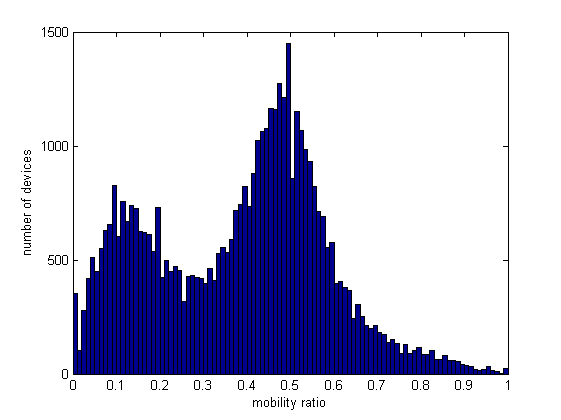
\includegraphics[scale=0.7]{mobility.png}
\captionsetup{justification=centering}
\caption{Histogram of mobility ratio of all devices in the wifilog}
\label{figure:mobility}
\end{figure}

\section{States to movements}\label{statesToMovements}
The data resulting from preprocessing contains the states of where a particular device was located during a certain time period. Implicitly this also includes information on the movement of the device. If a device is first located in building A and subsequently in building B it must have moved from building A to B. However, in order to be able to retrieve the movement patterns of devices the movement should be stored explicitly. This means that each record should store the movement of one device from one building to another building or to world. Examples of movement patterns that can be retrieved from this data are: the number of devices moving from building A to B within a given time period, and the peak in movement from the canteen to all other building-parts. 
To create records for each individual movement first the preprocessed data is ordered on mac address and start time. By doing this all the subsequent states for every device are listed directly below each other (see \autoref{figure:movementrecs}). As a movement is defined by the change of one state to another, movements records can be created from every two consecutive state records (see \autoref{figure:movementrecs}. However, not every two consecutive states represent a movement. Only when the two states concern the same device and they are at different buildings they represent a movement. This means that movement records with different mac addresses or similar building ids are filtered out (see \autoref{figure:movementrecs}. \autoref{figure:statesToMovements} shows the creation of movement records graphically. The states are shown in black, the movements in red.

\begin{figure}[H]
\centering
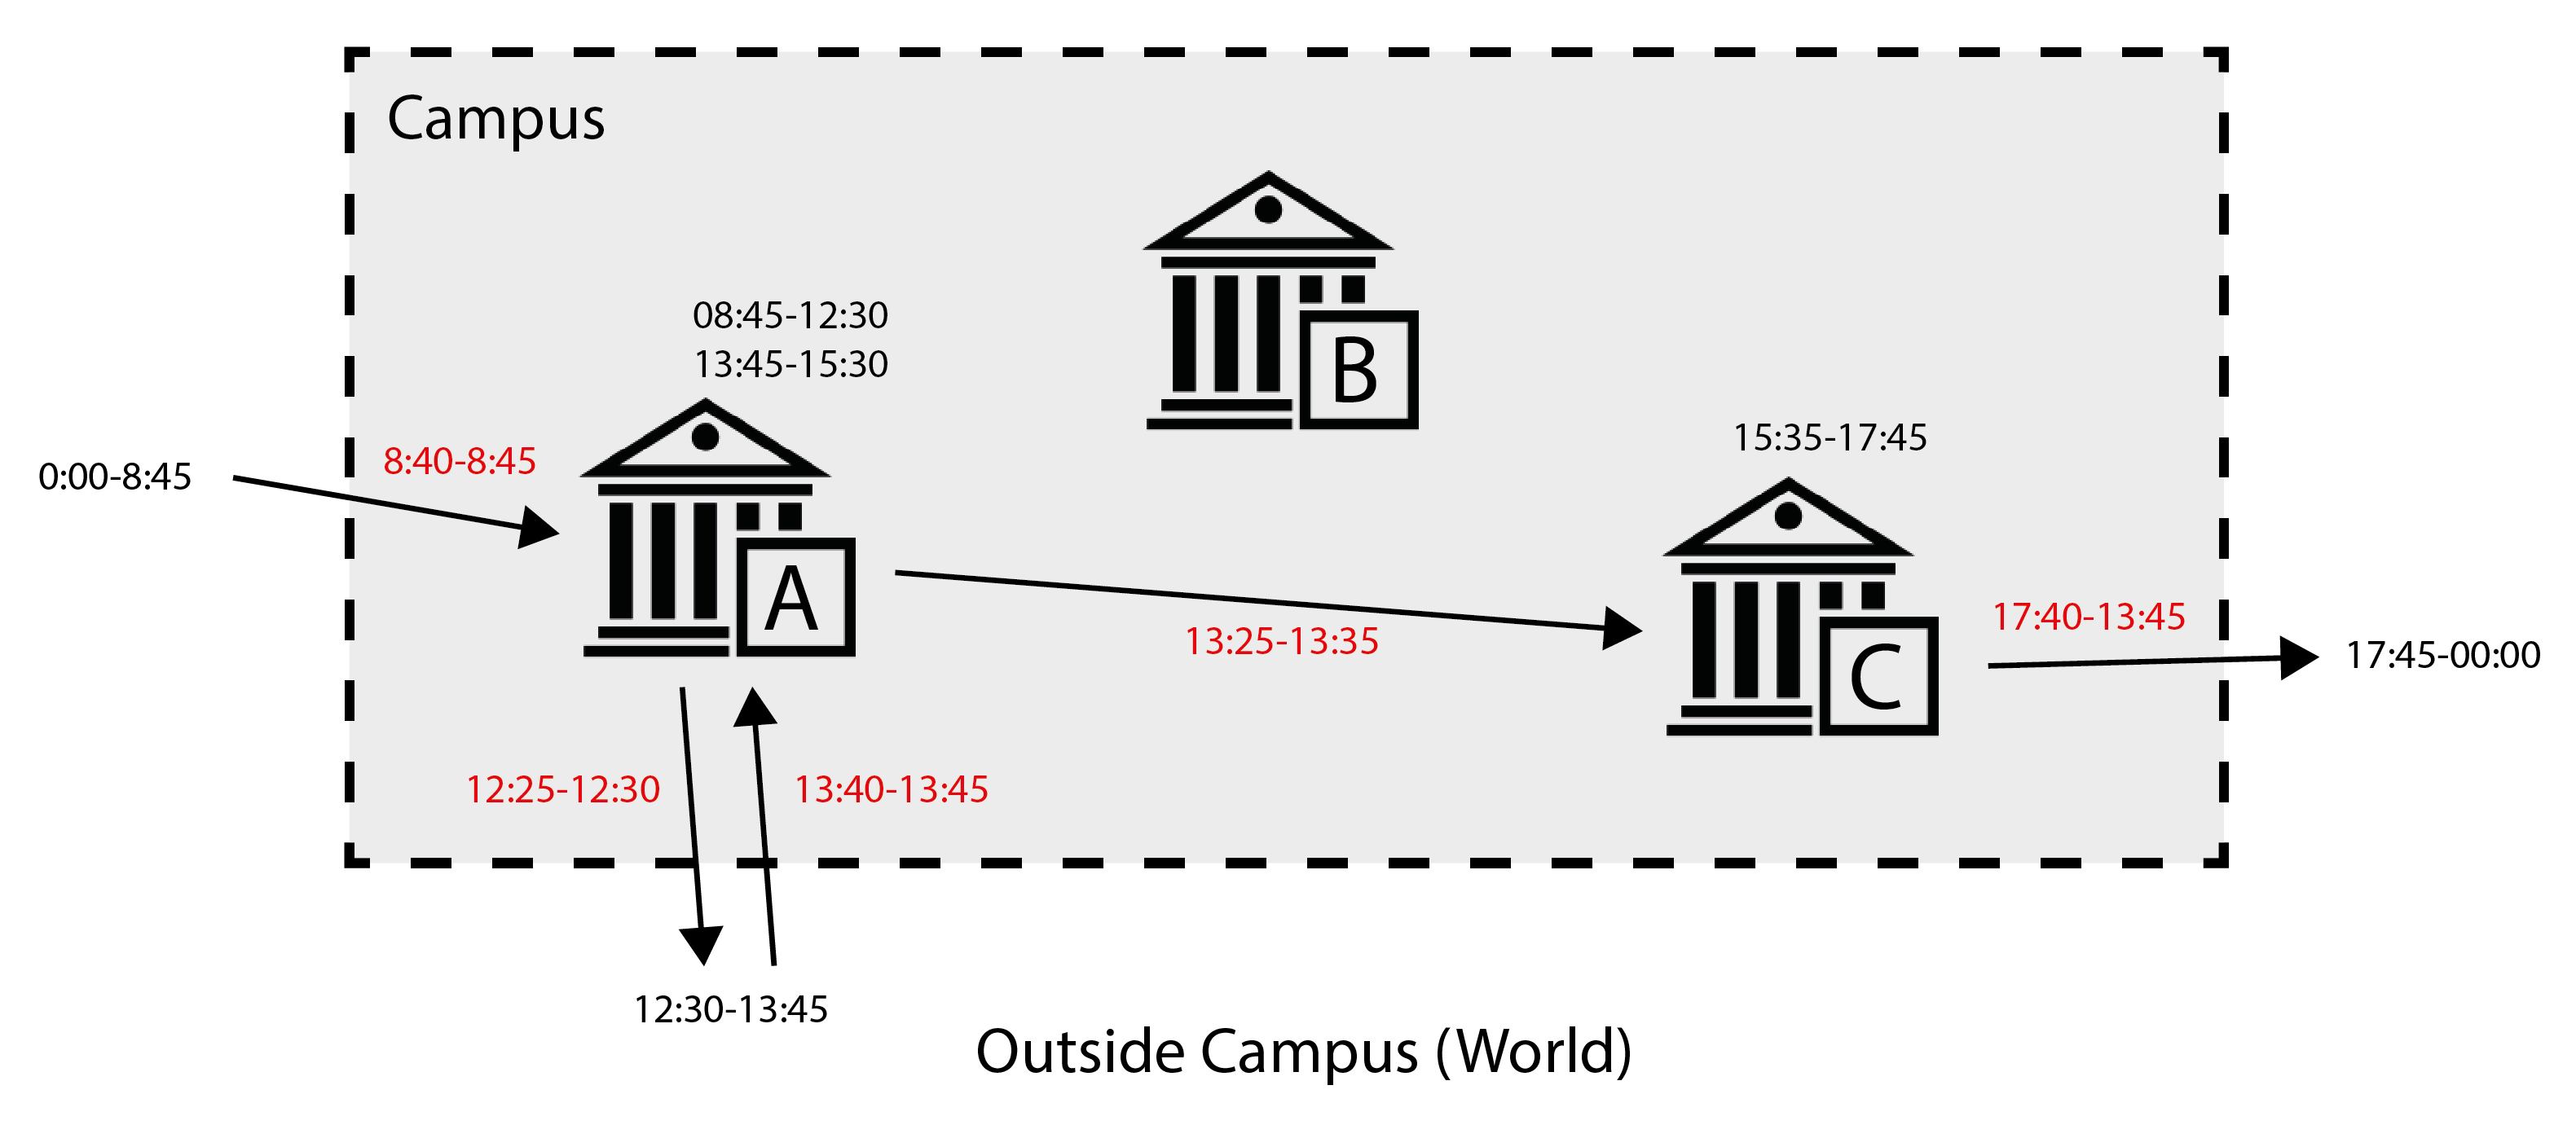
\includegraphics[scale=0.55]{statesToMovements.png}
\captionsetup{justification=centering}
\caption{Graphic representation; retrieving movements from states}
\label{figure:statesToMovements}
\end{figure}

\begin{figure}[H]
\centering
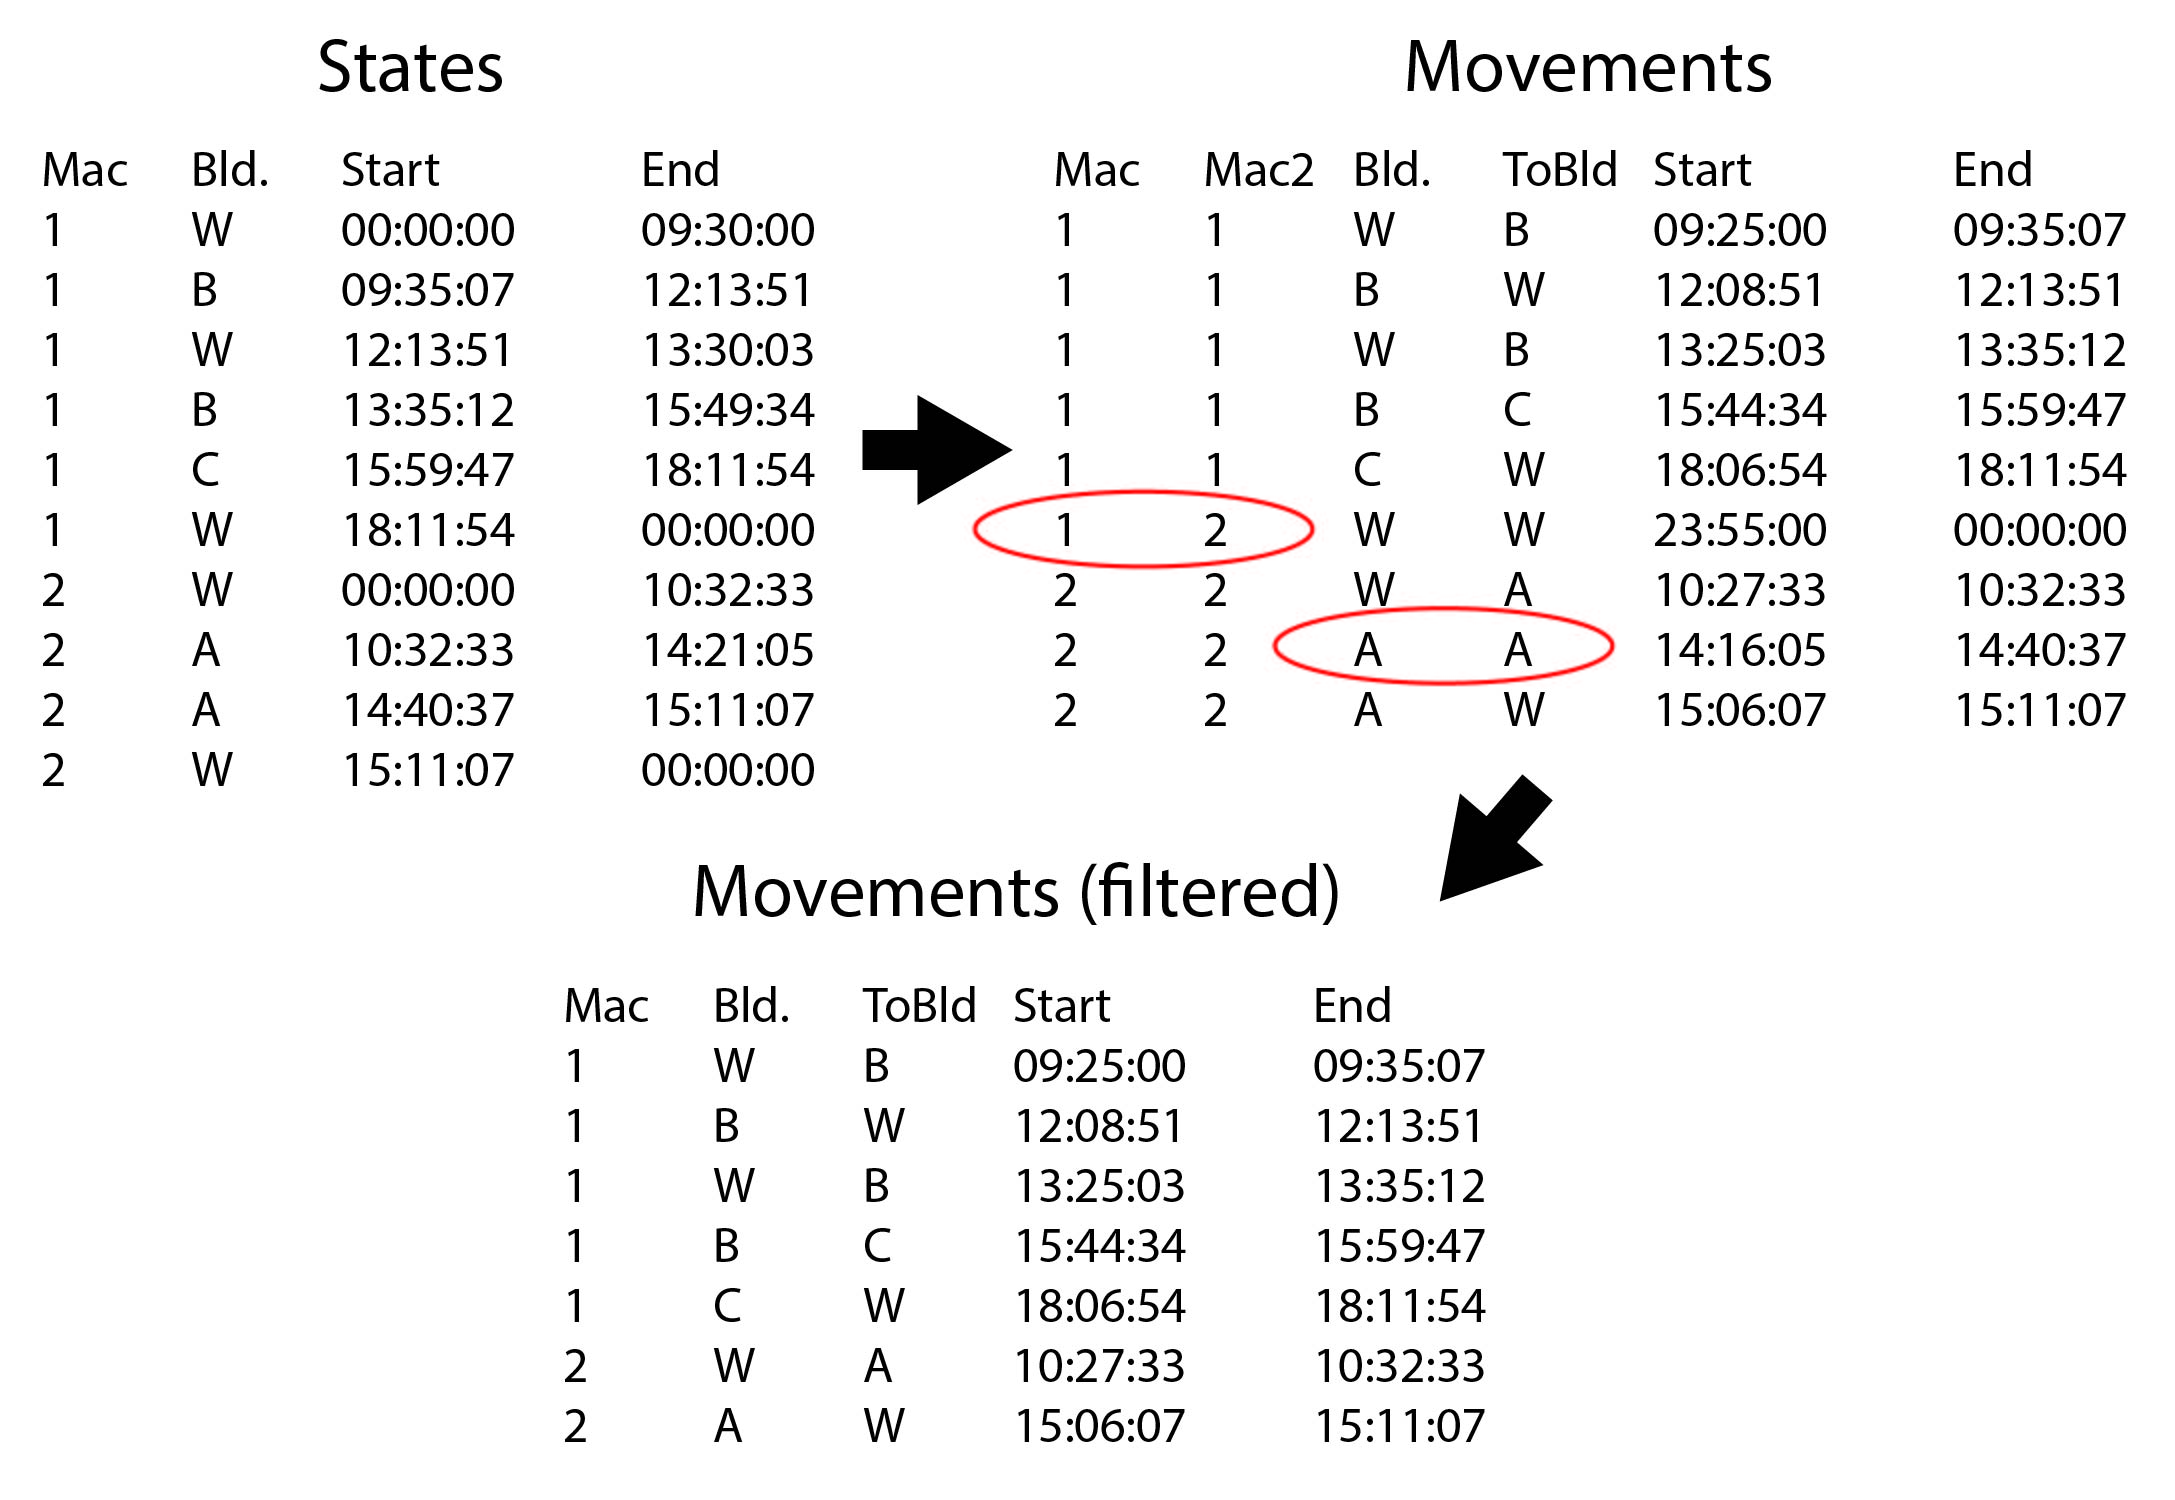
\includegraphics[scale=0.2]{movement_records.jpg}
\captionsetup{justification=centering}
\caption{Database representation; retrieving movements from states}
\label{figure:movementrecs}
\end{figure}

The start and end time of the movement are defined by the end time of the previous state minus 5 minutes, and the start time of the next state (see \autoref{figure:movement}). The reason that 5 minutes are subtracted from the end time of the previous state is that this is approximately the last moment in time the device was actually scanned at the location of the previous state. In the figure below the device is scanned 15:21 at building B. Approximately 5 minutes later (at 20:27) the device is scanned at building C. The state record of building B however continues all the way until 20:27, whilst the last time it was actually scanned at building B was 15:21. As a result it can be concluded that the movement from building B to C took place somewhere between 15:21 and 20:27. Therefore the start time of the movement between B and C can be approximated by subtracting 5 minutes from the end time of the state record at B. As can be observed in the movement from A to B is retrieved in the same way.

\begin{figure}[H]
\centering
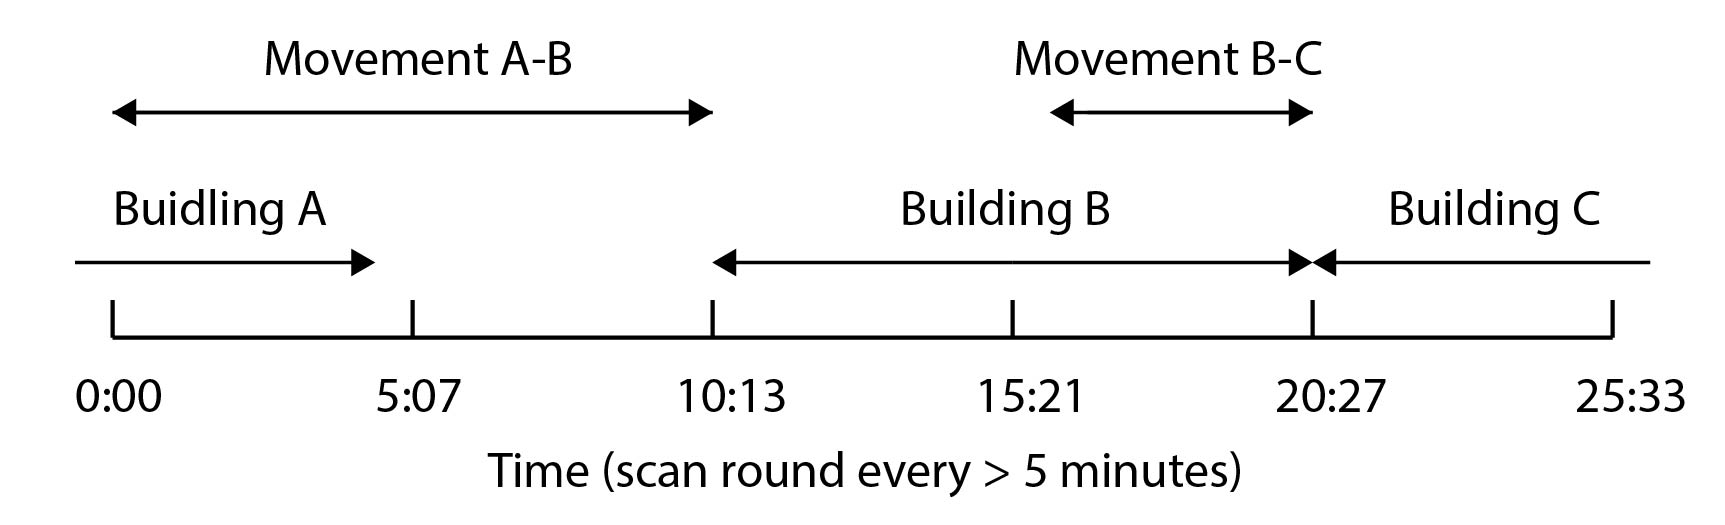
\includegraphics[scale=0.2]{movement.jpg}
\captionsetup{justification=centering}
\caption{Defining the start and end time of a single movement}
\label{figure:movement}
\end{figure}


\section{States to trajectories}\label{statesToTrajectories}
An individuals trajectory is constructed as a sequence of locations in order of the scan time. Start and end time of a trajectory can be specified with a time interval. Two consecutive scans from the Wi-Fi log are considered in the same trajectory if and only if \textit{$t_{s2}$ - $t_{e1}$} \textless \textit{$T_{split}$}, where \textit{$T_{split}$} is the splitting threshold. The splitting threshold is important when dealing with people, who are not observed for a long duration of time, i.e. people moving home. For example, if a student leaves the campus at the end of the day, and returns the next morning, separate trajectories should be created. Because, \textit{$T_{split}$} is larger than the threshold for identifying \textit{'world'} (see \autoref{preprocessing}), the trajectory will always start and end with \textit{'world'}. If \textit{p} is a location, then a trajectory can be written as:
$$p_{1} \rightarrow p_{2} \rightarrow p_{3} \rightarrow … \rightarrow p_{n}$$
Given a time interval, there is a set of individual trajectories $\textit{S} = \{t_{1}, t_{2}, t_{3},...,t_{n}\}$ where each $t_{i}$ is the trajectory.
